\documentclass[tikz]{standalone}
\input{../tikz/plots_config.pgs}

\begin{document}

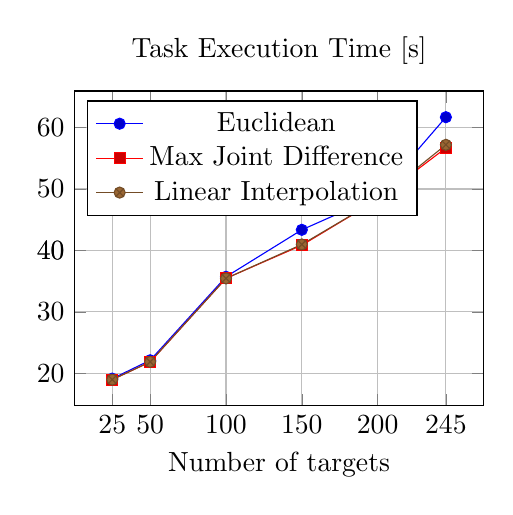
\begin{tikzpicture}
\begin{axis}[%
width=52mm,
height=40mm,
scale only axis,
xmin=0,
xmax=270,
xmajorgrids,
ymajorgrids,
xtick={25, 50, 100, 150, 200, 245},
ytick={10, 20, 30, 40, 40, 50, 60, 70},
title={Task Execution Time [s]},
xlabel={Number of targets},
legend pos=north west,
]
\addplot coordinates{
	(25, 19.1144768858)
	(50, 22.1051626324)
	(100, 35.7024459733)
	(150, 43.3519740802)
	(200, 48.8300051753)
	(245, 61.6969027166)
};
\addlegendentry{Euclidean};

\addplot coordinates{
	(25, 18.9472660486)
	(50, 21.8354147047)
	(100, 35.441645496)
	(150, 40.8434635126)
	(200, 48.2612611198)
	(245, 56.6949338939)
};
\addlegendentry{Max Joint Difference};

\addplot coordinates{
	(25, 18.9472660486)
	(50, 21.8482669676)
	(100, 35.4413149319)
	(150, 40.970932502)
	(200, 48.2612611198)
	(245, 57.1981783243)
};
\addlegendentry{Linear Interpolation};

\end{axis}
\end{tikzpicture}

\end{document}
